\documentclass{article}
\usepackage{graphicx}
\usepackage{caption}
\usepackage{subcaption}
\usepackage{hyperref}
\graphicspath{{./figs/}}{}
\usepackage{listings}
\title{
HLS-Assignment 8
}
\begin{document}
\maketitle
\hfill \textbf{Sampath Govardhan} \\
\null \hfill \textbf{FWC22071}\\
\maketitle
\hfill \textbf{VITIS-HLS}
\section{Problem Statement}
\begin{lstlisting}
HELLO
\end{lstlisting}
\vspace{6cm}
\section{Header File}
\begin{lstlisting}
#ifndef _HEADER_H_
#define _HEADER_H_

#include <hls_stream.h>
#include "ap_int.h"
using namespace std;
#define N 8  //8bits per clock cycle

typedef ap_uint<N> data;

void crc24a(hls::stream<data>& input, hls::stream<data>& output, ap_uint<1> last);

#endif


\end{lstlisting}

\vspace{15cm}
\section{CRC bits Generator Code}
\begin{lstlisting}
//crc.cpp
#include "header.h"

void crc24a(hls::stream<data>& input, hls::stream<data>& output, ap_uint<1> last) {

#pragma HLS INTERFACE mode=axis register_mode=both port=input register
#pragma HLS INTERFACE mode=axis register_mode=both port=output register
#pragma HLS INTERFACE mode=ap_none port=last

    ap_uint<1> divisor[25] = {1, 1, 0, 0, 0, 0, 1, 1, 0, 0, 1, 0, 0, 1, 1, 0, 0, 1, 1, 1, 1, 1, 0, 1, 1};

    int y = 25;  // loading Size of divisor array into a variable

    ap_uint<1> crc[32];

    int x = 32;  // Size of dividend array(len of input+divisor-1)

    // Read input stream a
    data d =input.read();
        for (int j = 0; j < 8; j++) {
#pragma HLS PIPELINE II=1
            crc[j]=d[j];
        }
    // Add padding zeros to dividend
    for (int i = 8; i < 32; i++) {
#pragma HLS PIPELINE II=1
        crc[i] = 0;
    }


    // Division is performed only when last is high
    for (int i = 0; i <= x - y; i++) {
#pragma HLS PIPELINE II=1
        if (crc[i] == 1  && last==1) {
            for (int j = 0; j < y; j++) {
#pragma HLS UNROLL
                crc[i + j] = crc[i+j] ^ divisor[j];
            }
        }
    }

    // Find start index of nonzero bits in dividend(crc)
    int startIdx = 0;
    while (startIdx < x && crc[startIdx] == 0) {
        startIdx++;
    }

   // Store nonzero values into another array
	ap_uint<1> f[24];

    for (int i = 0; i < 24; i++) {
#pragma HLS PIPELINE II=1
    	f[i] = (startIdx == x) ? crc[i] : crc[startIdx + i];
    }

   data g,h,m,o;

   for (int i = 0; i < 24; i++) {
#pragma HLS PIPELINE II=1
          if (i < 8) {
              o(i, i) = d(i, i);
              g(i, i) = f[i];
          } else if (i < 16) {
              h(i%8, i%8) = f[i];
          } else {
              m(i%8, i%8) = f[i];
          }
      }
   // Write the result to output stream c
    output.write(o);
    output.write(g);
    output.write(h);
    output.write(m);

}

\end{lstlisting}
\vspace{3cm}

\section{Test Bench Code}
\begin{lstlisting}
//crc_tb.cpp
#include "header.h"

int main() {
    hls::stream<data> a,b;
    data x, y;
    ap_uint<1> last;




      x=0b00010110;

          /* ap_uint<1> dividend[8] = {0, 1, 1, 0, 1, 0, 0, 0};
   	       for (int i = 0; i < 8; i++) {

   	              x(i,i) = dividend[i];

   	              }
   	      */

   	       a.write(x);
   	       last=1;



    // Perform binary divisdatan
    crc24a(a, b, last);

    // Read the result from the output stream out1
    cout << "CRC generator output : "<<endl;;
    ap_uint<1> p[32];


    for (int i = 0; i < 4; i++) {
        y = b.read();
        for (int j = 0; j < 8; j++) {
            p[i * 8 + j] = y(j, j);
        }
    }

    for (int i = 0; i < 32; i++) {
        cout << p[i];
    }

    cout<<endl;

    return 0;
}

\end{lstlisting}
\vspace{3cm}


\section{C simulation Output}
\begin{lstlisting}
INFO: [SIM 2] *************** CSIM start ***************
INFO: [SIM 4] CSIM will launch GCC as the compiler.
   Compiling ../../../../../codes/crc_tb.cpp in debug mode
   Compiling ../../../../../codes/crc.cpp in debug mode
   Generating csim.exe
CRC generator output : 
01101000101101001111001100000010
INFO [HLS SIM]: The maximum depth reached by any hls::stream() instance in the design is 4
INFO: [SIM 1] CSim done with 0 errors.
INFO: [SIM 3] *************** CSIM finish ***************



\end{lstlisting}
\vspace{10cm}



\section{HLS Resource Consumption Report}
\vspace{1cm}
\begin{figure}[h]
\centering
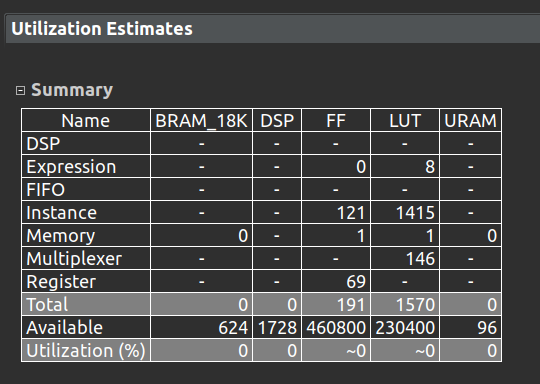
\includegraphics[width=\textwidth]{figs/1.png}
    \caption{CP Removal}
    \label{fig:my_label}
\end{figure}

\vspace{13cm}


\section{HLS Timing and Fmax Report}
\vspace{1cm}
\begin{figure}[h]
    \centering
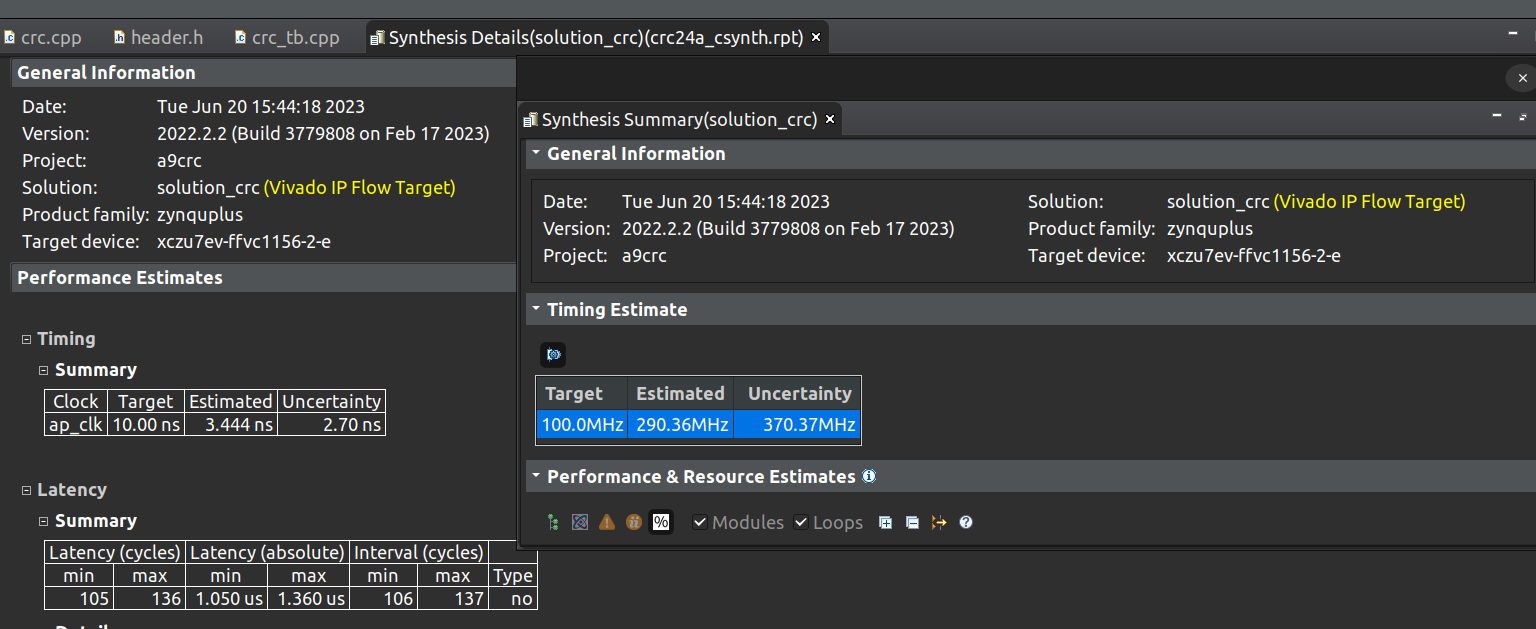
\includegraphics[width=\textwidth]{figs/2.png}
    \caption{CP Removal}
    \label{fig:my_label}
\end{figure}

\vspace{15cm}


\section{CoSimulation Report}
\vspace{1cm}
\begin{figure}[h]
    \centering
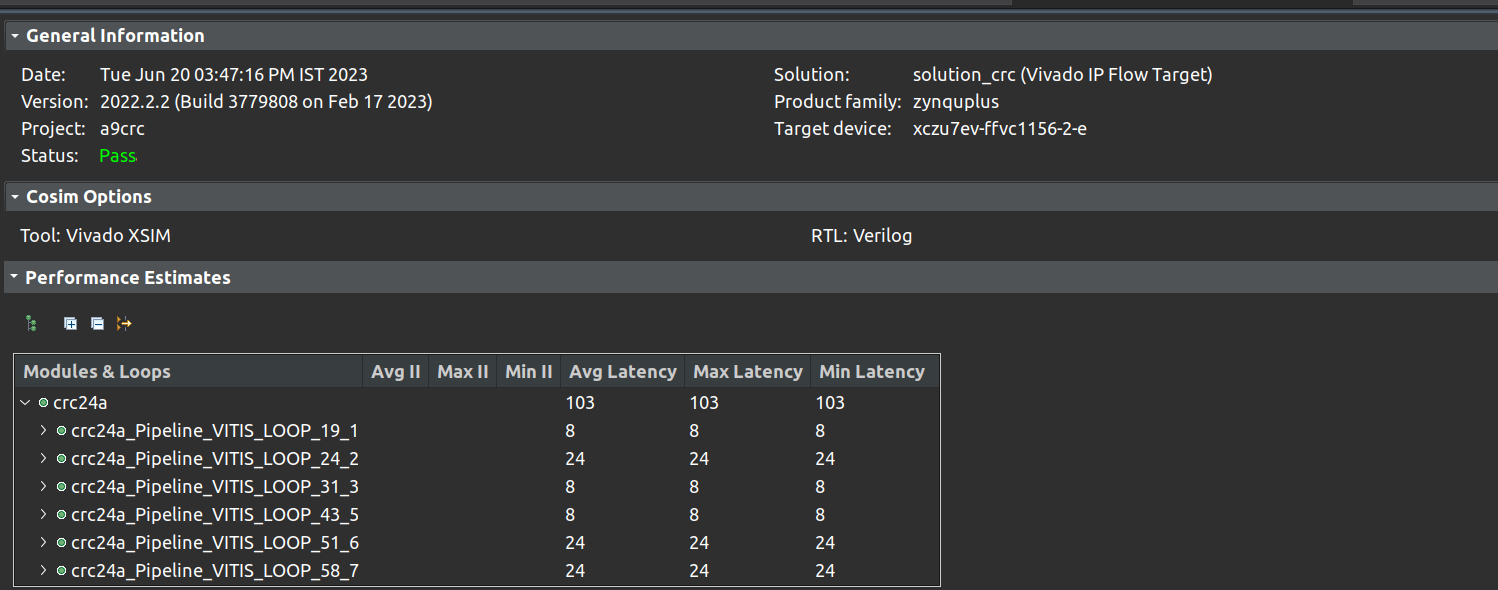
\includegraphics[width=\textwidth]{figs/3.png}
    \caption{CP Removal}
    \label{fig:my_label}
\end{figure}

\vspace{15cm}


\maketitle
\hfill \textbf{VIVADO}
\section{Block Design}
\vspace{1cm}
\begin{figure}[h]
    \centering
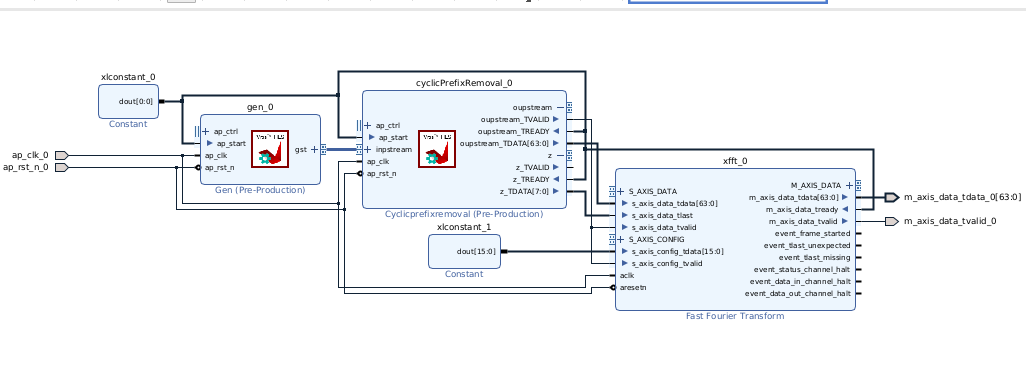
\includegraphics[width=\columnwidth]{figs/bd.png}
    \caption{Cosimulation Report}
    \label{fig:my_label}
\end{figure}
\vspace{3cm}
\section{Verilog Testbench}
\begin{lstlisting}
// Engineer: 
// 
// Create Date: 05/25/2023 11:59:07 AM
// Design Name: 
// Module Name: wav_tb
// Project Name: 
// Target Devices: 
// Tool Versions: 
// Description: 
// 
// Dependencies: 
// 
// Revision:
// Revision 0.01 - File Created
// Additional Comments:
// 
//////////////////////////////////////////////////////////////////////////////////


module wav_tb(

    );
    
  reg clk; 
  reg rst;
  wire [63:0]m_axis_data_tdata_0;
  wire m_axis_data_tvalid_0;
  integer file;
  reg [31:0] sample_counter;

  design_1_wrapper i
       (.ap_clk_0(clk),
        .ap_rst_n_0(rst),
        .m_axis_data_tdata_0(m_axis_data_tdata_0),
        .m_axis_data_tvalid_0(m_axis_data_tvalid_0));
        

                                       
        always #5 clk=~clk;
        initial begin
        
        rst=0;clk=1;
        #100 rst=1;
        #89130000 $finish;
        end      
        
        initial begin
        
        file=$fopen("fft_output_vivadoip.txt","w");
        sample_counter = 0;

    while (sample_counter < 8192) begin
      #10;  // Assuming a sampling rate of 10 units

        if (m_axis_data_tvalid_0) begin
         $fwrite(file, "%h\n", m_axis_data_tdata_0);
        sample_counter = sample_counter + 1;
      end
    end

    $fclose(file);
  end
endmodule

\end{lstlisting}

\vspace{3cm}


\section{Output Waveform}
\vspace{1cm}
\begin{figure}[h]
\centering
\begin{subfigure}[b]{1.2\textwidth}
    \centering
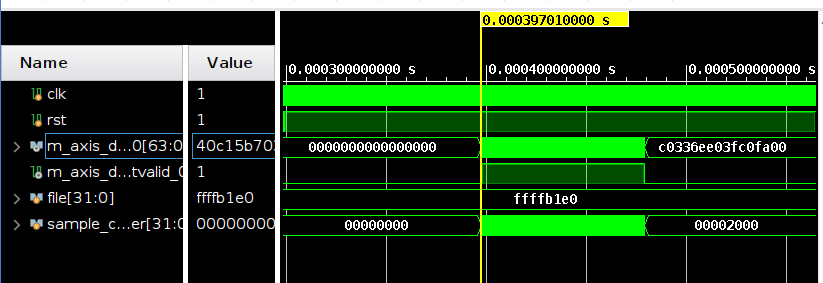
\includegraphics[width=\textwidth]{figs/wav1.png}
    \caption{output of FFT}
    \label{fig:my_label}
\end{subfigure}
\hfill
\begin{subfigure}[b]{1.2\textwidth}
    \centering
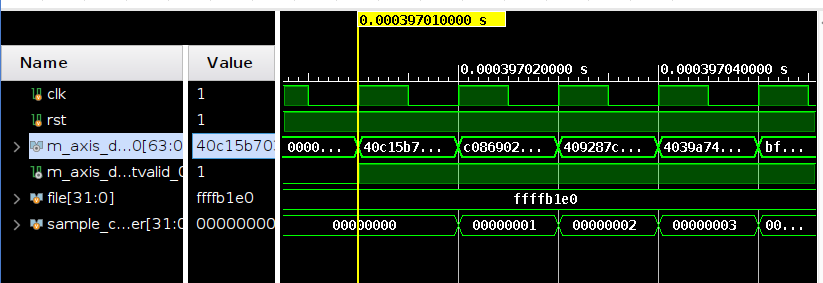
\includegraphics[width=\textwidth]{figs/wav2.png}
    \caption{Zoomed format of above figure}
    \label{fig:my_label}
\end{subfigure}
\end{figure}
\vspace{15cm}

\maketitle
\hfill \textbf{MATLAB}
\section{Matlab Code}
\begin{lstlisting}
clc;
close all;
x = [complex(-0.601084,-0.059909) complex(0.571592,0.530777) complex(0.096652,-0.704768) complex(-0.493203,0.428746) 
X = fft(x);

disp('FFT Output:');
disp(X);

fileID = fopen('fft_output_matlab.txt', 'w');
fprintf(fileID, 'Real \t Imaginary \n');
for k = 1:length(X)
    fprintf(fileID, '%d \t %d \n', real(X(k)), imag(X(k)));
end
fclose(fileID);

\end{lstlisting}
\vspace{3cm}
\section{Conclusion}
\begin{lstlisting}
The Output of FFTIP is matching with Output of Matlab with Precision 
using this floating Point Converter Online :

\end{lstlisting}
\url{https://www.h-schmidt.net/FloatConverter/IEEE754.html}
\vspace{4cm}
\\
\textbf{GITHUB :} \url{https://github.com/dk-425/Training.git}
\end{document}


